\section{Application Acceleration}
\label{sec:acceleration}

In this section, we demonstrate the performance and benefits of the FlashBoost
architecture by presenting some simple accelerator examples. 

\subsection{Nearest Neighbor Search}

Nearest neighbor search is a classical problem with many applications. One of
the modern achievements in this field is Locality Sensitive Hashing~\cite{lsh}.
LSH hashes the dataset using multiple hash functions, so that
similar data is statistically likely to be hashed to similar buckets. When
querying, the query is hashed using the same hash functions, and only the data
in the matching buckets are actually compared. The bulk of the work during a
query process is traversing hash buckets and reading the corresponding data to
perform distance calculation. Because data pointed to by the hash buckets are
most likely scattered across the dataset, access patterns are heavily random.

We have built a LSH query accelerator, where all of the data is stored in flash
and the distance calculation is done by the in-storage processor on the storage
device. For simplicity, we assume 8KB data items, and calculate the hamming
distance between the query data and each of the items in the has bucket. The
software sends a stream of addresses from a hash bucket along with the query
data, and the system will return the index of the item most closely matching the
query. By offloading computation to the in-storage accelerator, we
show XXX\% performance improvement over the non-accelerated implementation.



\subsection{Graph Traversal}

Efficient graph traversal is a very important component of any graph processing
system. It is also a very latency-bound problem because one often cannot predict
the next node to visit, until the previous node is visited and processed. We
demonstrate the performance benefits of our FlashBoost architecture by
implementing graph traversal that takes advantages of the in-storage processor
and the integrated storage network, which allows extremely low-latency access
into both local and remote flash storage. We demonstrate that compared to a
naive implementation that uses flash only as a storage device, we have XXX\%
performance improvement.

\begin{figure}[h]
	\begin{center}
	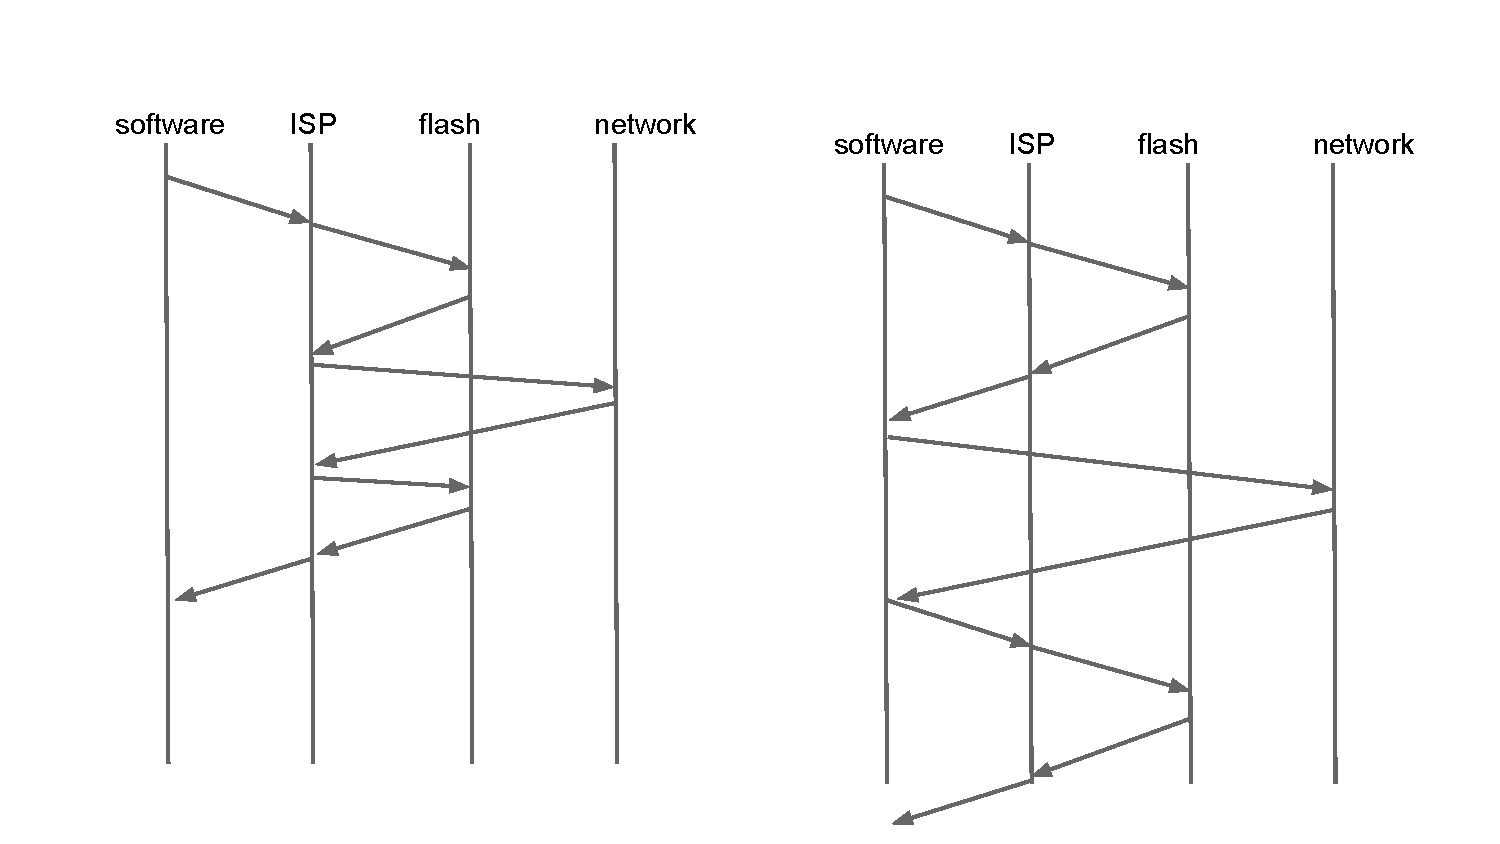
\includegraphics[width=0.4\paperwidth]{figures/graph_accel.pdf}
	\caption{Graph Traversal Comparison}
	\label{fig:graph_accel}
	\end{center}
\end{figure}

\subsection{Hardware-Accelerated String Search}

We implemented a hardware-accelerated string search that interacts with the file
system. Our file system is modified so that it can provide the physical location
of each file to the user software. The user software consults the file system for the locations of a
particular file, and streams the list of physical addresses to the in-store
processor. The in-store processor can read the files from flash, perform string
search using a hardware accelerator, and return only the results back to the
user software. 

This example demonstrates that our in-storage processor platform can easily be
used in conjunction with the high-level file system, so that the developer does
not have to deal with high level issues like file layout and permissions while
not sacrificing performance.

Ming and Sungjin writing string search
